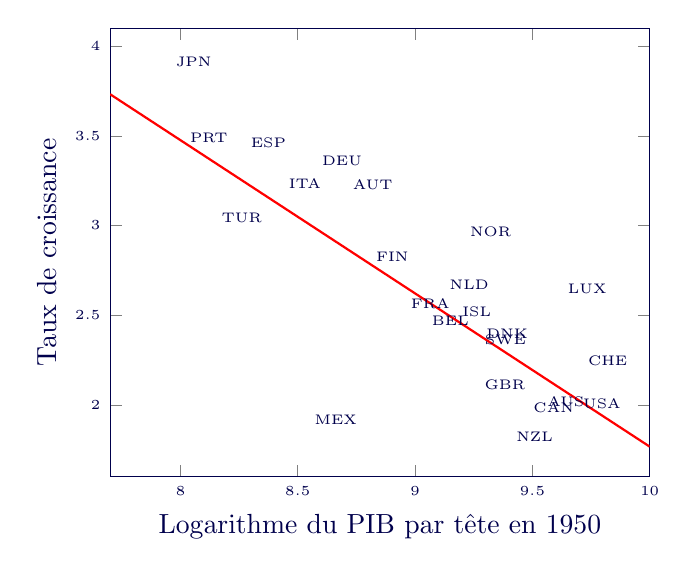
\begin{tikzpicture}
\tikzstyle{every node}=[font=\tiny]
\begin{axis}[
enlargelimits=false, color=blue!30!black,
scale=1,
xmin=7.7,
xmax=10,
xlabel style={font=\color{white!15!black}},
xlabel={Logarithme du PIB par tête en 1950},
ymin=1.6,
ymax=4.1,
ylabel style={font=\color{white!15!black}},
ylabel={Taux de croissance},
axis background/.style={fill=white}
]
\addplot[draw=red, thick, smooth, samples=2, domain=7.7:10,]{10.3117-0.8545*x} ;
\node[right, align=left] at (axis cs:9.522,2.016) {AUS};
\node[right, align=left] at (axis cs:8.693,3.227) {AUT};
\node[right, align=left] at (axis cs:9.03,2.466) {BEL};
\node[right, align=left] at (axis cs:9.463,1.982) {CAN};
\node[right, align=left] at (axis cs:9.696,2.247) {CHE};
\node[right, align=left] at (axis cs:8.562,3.362) {DEU};
\node[right, align=left] at (axis cs:9.262,2.398) {DNK};
\node[right, align=left] at (axis cs:8.258,3.461) {ESP};
\node[right, align=left] at (axis cs:8.792,2.823) {FIN};
\node[right, align=left] at (axis cs:8.94,2.563) {FRA};
\node[right, align=left] at (axis cs:9.255,2.113) {GBR};
\node[right, align=left] at (axis cs:9.16,2.521) {ISL};
\node[right, align=left] at (axis cs:8.42,3.232) {ITA};
\node[right, align=left] at (axis cs:7.939,3.915) {JPN};
\node[right, align=left] at (axis cs:9.61,2.647) {LUX};
\node[right, align=left] at (axis cs:8.53,1.914) {MEX};
\node[right, align=left] at (axis cs:9.106,2.672) {NLD};
\node[right, align=left] at (axis cs:9.193,2.963) {NOR};
\node[right, align=left] at (axis cs:9.39,1.82) {NZL};
\node[right, align=left] at (axis cs:7.999,3.491) {PRT};
\node[right, align=left] at (axis cs:9.256,2.363) {SWE};
\node[right, align=left] at (axis cs:8.134,3.042) {TUR};
\node[right, align=left] at (axis cs:9.675,2.005) {USA};
\end{axis}
\end{tikzpicture}%